\documentclass[1p]{elsarticle_modified}
%\bibliographystyle{elsarticle-num}

%\usepackage[colorlinks]{hyperref}
%\usepackage{abbrmath_seonhwa} %\Abb, \Ascr, \Acal ,\Abf, \Afrak
\usepackage{amsfonts}
\usepackage{amssymb}
\usepackage{amsmath}
\usepackage{amsthm}
\usepackage{scalefnt}
\usepackage{amsbsy}
\usepackage{kotex}
\usepackage{caption}
\usepackage{subfig}
\usepackage{color}
\usepackage{graphicx}
\usepackage{xcolor} %% white, black, red, green, blue, cyan, magenta, yellow
\usepackage{float}
\usepackage{setspace}
\usepackage{hyperref}

\usepackage{tikz}
\usetikzlibrary{arrows}

\usepackage{multirow}
\usepackage{array} % fixed length table
\usepackage{hhline}

%%%%%%%%%%%%%%%%%%%%%
\makeatletter
\renewcommand*\env@matrix[1][\arraystretch]{%
	\edef\arraystretch{#1}%
	\hskip -\arraycolsep
	\let\@ifnextchar\new@ifnextchar
	\array{*\c@MaxMatrixCols c}}
\makeatother %https://tex.stackexchange.com/questions/14071/how-can-i-increase-the-line-spacing-in-a-matrix
%%%%%%%%%%%%%%%

\usepackage[normalem]{ulem}

\newcommand{\msout}[1]{\ifmmode\text{\sout{\ensuremath{#1}}}\else\sout{#1}\fi}
%SOURCE: \msout is \stkout macro in https://tex.stackexchange.com/questions/20609/strikeout-in-math-mode

\newcommand{\cancel}[1]{
	\ifmmode
	{\color{red}\msout{#1}}
	\else
	{\color{red}\sout{#1}}
	\fi
}

\newcommand{\add}[1]{
	{\color{blue}\uwave{#1}}
}

\newcommand{\replace}[2]{
	\ifmmode
	{\color{red}\msout{#1}}{\color{blue}\uwave{#2}}
	\else
	{\color{red}\sout{#1}}{\color{blue}\uwave{#2}}
	\fi
}

\newcommand{\Sol}{\mathcal{S}} %segment
\newcommand{\D}{D} %diagram
\newcommand{\A}{\mathcal{A}} %arc


%%%%%%%%%%%%%%%%%%%%%%%%%%%%%5 test

\def\sl{\operatorname{\textup{SL}}(2,\Cbb)}
\def\psl{\operatorname{\textup{PSL}}(2,\Cbb)}
\def\quan{\mkern 1mu \triangleright \mkern 1mu}

\theoremstyle{definition}
\newtheorem{thm}{Theorem}[section]
\newtheorem{prop}[thm]{Proposition}
\newtheorem{lem}[thm]{Lemma}
\newtheorem{ques}[thm]{Question}
\newtheorem{cor}[thm]{Corollary}
\newtheorem{defn}[thm]{Definition}
\newtheorem{exam}[thm]{Example}
\newtheorem{rmk}[thm]{Remark}
\newtheorem{alg}[thm]{Algorithm}

\newcommand{\I}{\sqrt{-1}}
\begin{document}

%\begin{frontmatter}
%
%\title{Boundary parabolic representations of knots up to 8 crossings}
%
%%% Group authors per affiliation:
%\author{Yunhi Cho} 
%\address{Department of Mathematics, University of Seoul, Seoul, Korea}
%\ead{yhcho@uos.ac.kr}
%
%
%\author{Seonhwa Kim} %\fnref{s_kim}}
%\address{Center for Geometry and Physics, Institute for Basic Science, Pohang, 37673, Korea}
%\ead{ryeona17@ibs.re.kr}
%
%\author{Hyuk Kim}
%\address{Department of Mathematical Sciences, Seoul National University, Seoul 08826, Korea}
%\ead{hyukkim@snu.ac.kr}
%
%\author{Seokbeom Yoon}
%\address{Department of Mathematical Sciences, Seoul National University, Seoul, 08826,  Korea}
%\ead{sbyoon15@snu.ac.kr}
%
%\begin{abstract}
%We find all boundary parabolic representation of knots up to 8 crossings.
%
%\end{abstract}
%\begin{keyword}
%    \MSC[2010] 57M25 
%\end{keyword}
%
%\end{frontmatter}

%\linenumbers
%\tableofcontents
%
\newcommand\colored[1]{\textcolor{white}{\rule[-0.35ex]{0.8em}{1.4ex}}\kern-0.8em\color{red} #1}%
%\newcommand\colored[1]{\textcolor{white}{ #1}\kern-2.17ex	\textcolor{white}{ #1}\kern-1.81ex	\textcolor{white}{ #1}\kern-2.15ex\color{red}#1	}

{\Large $\underline{12a_{0004}~(K12a_{0004})}$}

\setlength{\tabcolsep}{10pt}
\renewcommand{\arraystretch}{1.6}
\vspace{1cm}\begin{tabular}{m{100pt}>{\centering\arraybackslash}m{274pt}}
\multirow{5}{120pt}{
	\centering
	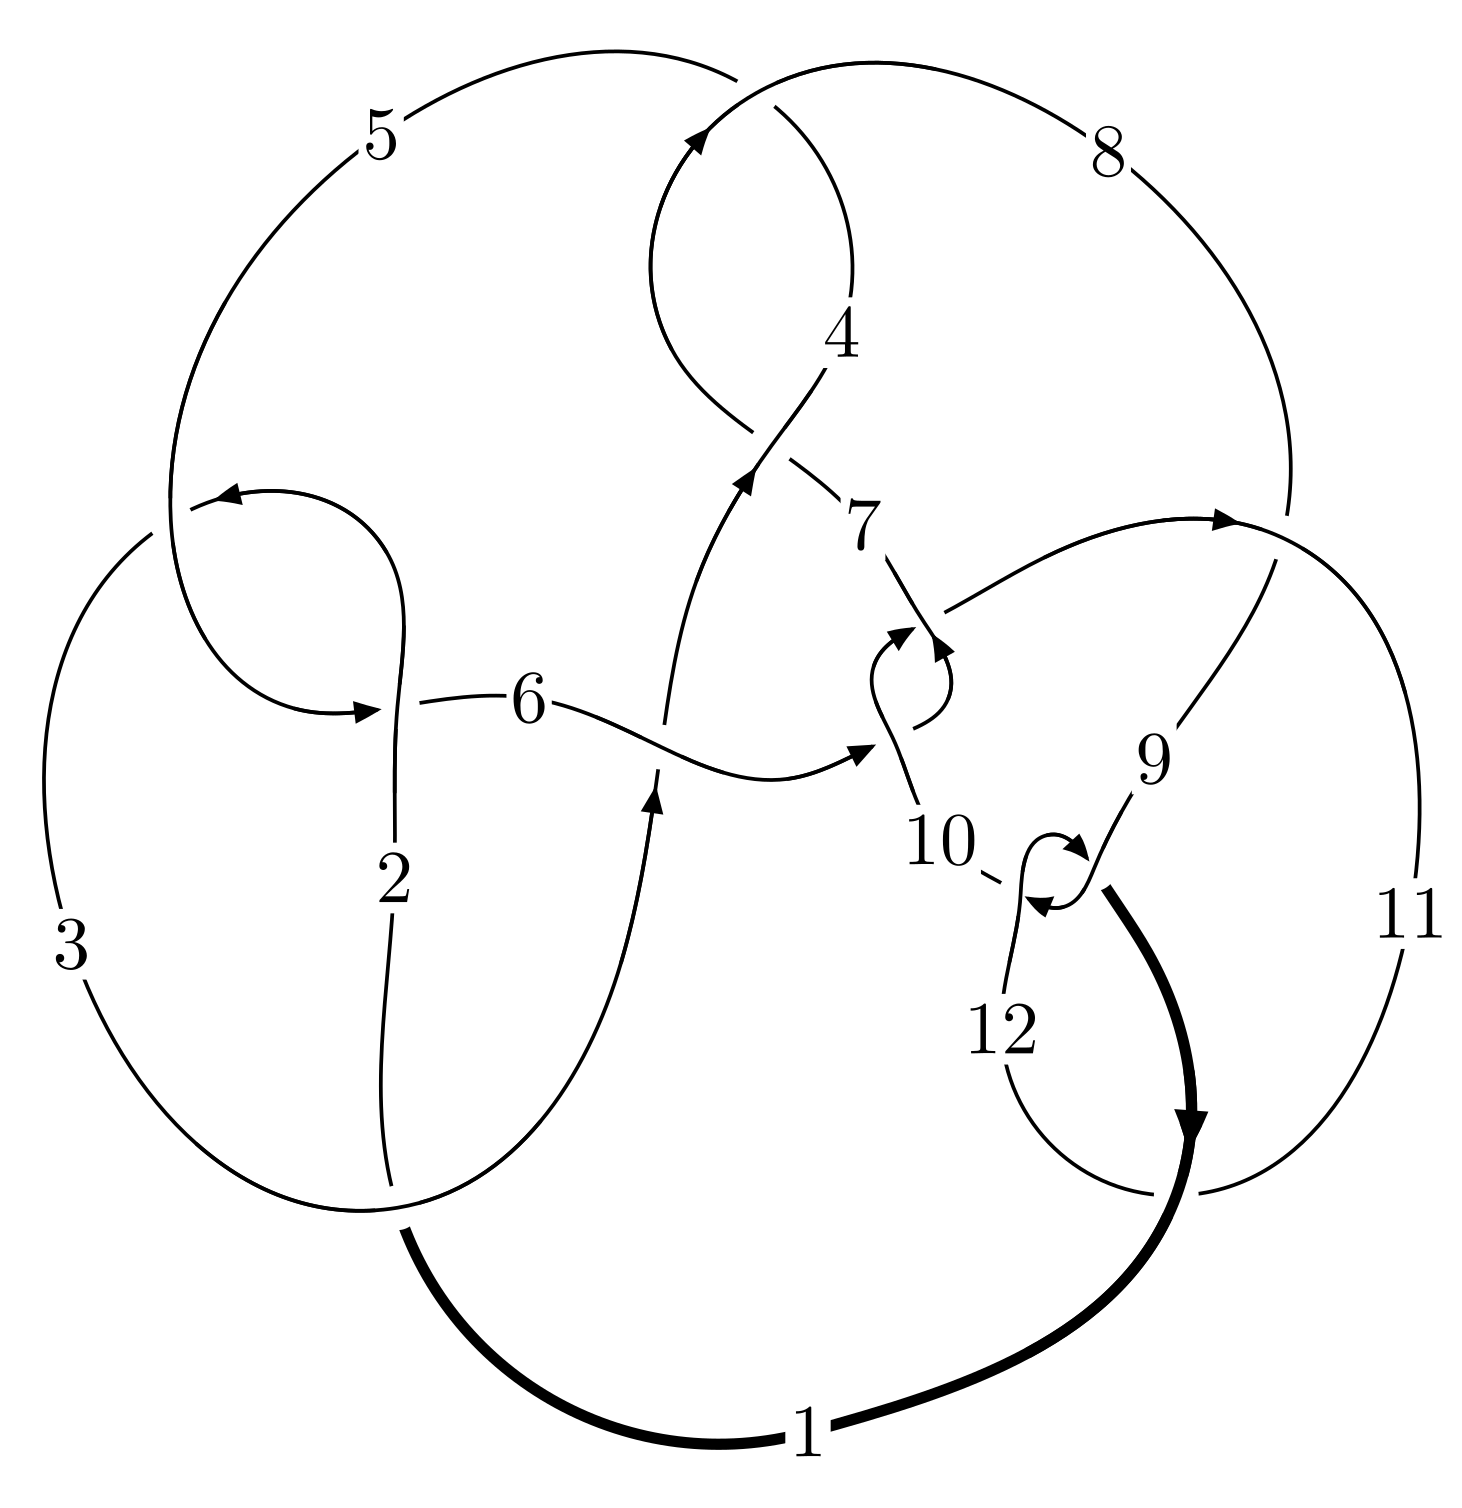
\includegraphics[width=112pt]{../../../GIT/diagram.site/Diagrams/png/805_12a_0004.png}\\
\ \ \ A knot diagram\footnotemark}&
\allowdisplaybreaks
\textbf{Linearized knot diagam} \\
\cline{2-2}
 &
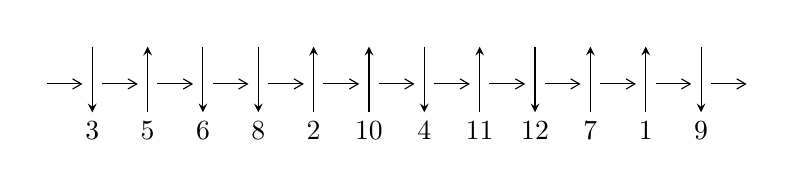
\begin{tikzpicture}[x=20pt, y=17pt]
	% nodes
	\node (C0) at (0, 0) {};
	\node (C1) at (1, 0) {};
	\node (C1U) at (1, +1) {};
	\node (C1D) at (1, -1) {3};

	\node (C2) at (2, 0) {};
	\node (C2U) at (2, +1) {};
	\node (C2D) at (2, -1) {5};

	\node (C3) at (3, 0) {};
	\node (C3U) at (3, +1) {};
	\node (C3D) at (3, -1) {6};

	\node (C4) at (4, 0) {};
	\node (C4U) at (4, +1) {};
	\node (C4D) at (4, -1) {8};

	\node (C5) at (5, 0) {};
	\node (C5U) at (5, +1) {};
	\node (C5D) at (5, -1) {2};

	\node (C6) at (6, 0) {};
	\node (C6U) at (6, +1) {};
	\node (C6D) at (6, -1) {10};

	\node (C7) at (7, 0) {};
	\node (C7U) at (7, +1) {};
	\node (C7D) at (7, -1) {4};

	\node (C8) at (8, 0) {};
	\node (C8U) at (8, +1) {};
	\node (C8D) at (8, -1) {11};

	\node (C9) at (9, 0) {};
	\node (C9U) at (9, +1) {};
	\node (C9D) at (9, -1) {12};

	\node (C10) at (10, 0) {};
	\node (C10U) at (10, +1) {};
	\node (C10D) at (10, -1) {7};

	\node (C11) at (11, 0) {};
	\node (C11U) at (11, +1) {};
	\node (C11D) at (11, -1) {1};

	\node (C12) at (12, 0) {};
	\node (C12U) at (12, +1) {};
	\node (C12D) at (12, -1) {9};
	\node (C13) at (13, 0) {};

	% arrows
	\draw[->,>={angle 60}]
	(C0) edge (C1) (C1) edge (C2) (C2) edge (C3) (C3) edge (C4) (C4) edge (C5) (C5) edge (C6) (C6) edge (C7) (C7) edge (C8) (C8) edge (C9) (C9) edge (C10) (C10) edge (C11) (C11) edge (C12) (C12) edge (C13) ;	\draw[->,>=stealth]
	(C1U) edge (C1D) (C2D) edge (C2U) (C3U) edge (C3D) (C4U) edge (C4D) (C5D) edge (C5U) (C6D) edge (C6U) (C7U) edge (C7D) (C8D) edge (C8U) (C9U) edge (C9D) (C10D) edge (C10U) (C11D) edge (C11U) (C12U) edge (C12D) ;
	\end{tikzpicture} \\
\hhline{~~} \\& 
\textbf{Solving Sequence} \\ \cline{2-2} 
 &
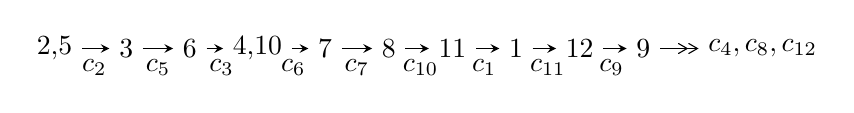
\begin{tikzpicture}[x=23pt, y=7pt]
	% node
	\node (A0) at (-1/8, 0) {2,5};
	\node (A1) at (1, 0) {3};
	\node (A2) at (2, 0) {6};
	\node (A3) at (49/16, 0) {4,10};
	\node (A4) at (33/8, 0) {7};
	\node (A5) at (41/8, 0) {8};
	\node (A6) at (49/8, 0) {11};
	\node (A7) at (57/8, 0) {1};
	\node (A8) at (65/8, 0) {12};
	\node (A9) at (73/8, 0) {9};
	\node (C1) at (1/2, -1) {$c_{2}$};
	\node (C2) at (3/2, -1) {$c_{5}$};
	\node (C3) at (5/2, -1) {$c_{3}$};
	\node (C4) at (29/8, -1) {$c_{6}$};
	\node (C5) at (37/8, -1) {$c_{7}$};
	\node (C6) at (45/8, -1) {$c_{10}$};
	\node (C7) at (53/8, -1) {$c_{1}$};
	\node (C8) at (61/8, -1) {$c_{11}$};
	\node (C9) at (69/8, -1) {$c_{9}$};
	\node (A10) at (11, 0) {$c_{4},c_{8},c_{12}$};

	% edge
	\draw[->,>=stealth]	
	(A0) edge (A1) (A1) edge (A2) (A2) edge (A3) (A3) edge (A4) (A4) edge (A5) (A5) edge (A6) (A6) edge (A7) (A7) edge (A8) (A8) edge (A9) ;
	\draw[->>,>={angle 60}]	
	(A9) edge (A10);
\end{tikzpicture} \\ 

\end{tabular} \\

\footnotetext{
The image of knot diagram is generated by the software ``\textbf{Draw programme}" developed by Andrew Bartholomew(\url{http://www.layer8.co.uk/maths/draw/index.htm\#Running-draw}), where we modified some parts for our purpose(\url{https://github.com/CATsTAILs/LinksPainter}).
}\phantom \\ \newline 
\centering \textbf{Ideals for irreducible components\footnotemark of $X_{\text{par}}$} 
 
\begin{align*}
I^u_{1}&=\langle 
-5.58623\times10^{76} u^{129}-4.47141\times10^{78} u^{128}+\cdots+1.43114\times10^{77} b-2.84585\times10^{78},\\
\phantom{I^u_{1}}&\phantom{= \langle  }-6.57135\times10^{77} u^{129}+2.71715\times10^{77} u^{128}+\cdots+2.86227\times10^{77} a-1.19729\times10^{78},\\
\phantom{I^u_{1}}&\phantom{= \langle  }u^{130}-8 u^{129}+\cdots+2 u+1\rangle \\
I^u_{2}&=\langle 
a^4 u- a^3 u- a^3+a^2-2 a u+b- a+u+1,\;a^5+a^4 u- a^3 u- a^3-2 a^2- a u- u-1,\;u^2+u+1\rangle \\
I^u_{3}&=\langle 
b- a,\;u^4 a- u^3 a-2 u^4+u^2 a+2 u^3+a^2-2 u^2- a- u+2,\;u^5- u^4+2 u^3- u^2+u-1\rangle \\
\\
\end{align*}
\raggedright * 3 irreducible components of $\dim_{\mathbb{C}}=0$, with total 150 representations.\\
\footnotetext{All coefficients of polynomials are rational numbers. But the coefficients are sometimes approximated in decimal forms when there is not enough margin.}
\newpage
\renewcommand{\arraystretch}{1}
\centering \section*{I. $I^u_{1}= \langle -5.59\times10^{76} u^{129}-4.47\times10^{78} u^{128}+\cdots+1.43\times10^{77} b-2.85\times10^{78},\;-6.57\times10^{77} u^{129}+2.72\times10^{77} u^{128}+\cdots+2.86\times10^{77} a-1.20\times10^{78},\;u^{130}-8 u^{129}+\cdots+2 u+1 \rangle$}
\flushleft \textbf{(i) Arc colorings}\\
\begin{tabular}{m{7pt} m{180pt} m{7pt} m{180pt} }
\flushright $a_{2}=$&$\begin{pmatrix}1\\0\end{pmatrix}$ \\
\flushright $a_{5}=$&$\begin{pmatrix}0\\u\end{pmatrix}$ \\
\flushright $a_{3}=$&$\begin{pmatrix}1\\- u^2\end{pmatrix}$ \\
\flushright $a_{6}=$&$\begin{pmatrix}u\\u\end{pmatrix}$ \\
\flushright $a_{4}=$&$\begin{pmatrix}u^4+u^2+1\\u^4\end{pmatrix}$ \\
\flushright $a_{10}=$&$\begin{pmatrix}2.29585 u^{129}-0.949298 u^{128}+\cdots+20.9609 u+4.18300\\0.390335 u^{129}+31.2438 u^{128}+\cdots+51.6062 u+19.8853\end{pmatrix}$ \\
\flushright $a_{7}=$&$\begin{pmatrix}10.7738 u^{129}-82.0527 u^{128}+\cdots-10.7181 u-6.86334\\12.5299 u^{129}-88.0806 u^{128}+\cdots+9.84424 u+0.206116\end{pmatrix}$ \\
\flushright $a_{8}=$&$\begin{pmatrix}1.31653 u^{129}+0.669349 u^{128}+\cdots+12.0408 u+4.48855\\-1.36092 u^{129}+42.7776 u^{128}+\cdots+62.9324 u+23.3661\end{pmatrix}$ \\
\flushright $a_{11}=$&$\begin{pmatrix}-0.0358964 u^{129}+12.9188 u^{128}+\cdots+19.8042 u+2.41846\\-5.51164 u^{129}+63.3209 u^{128}+\cdots+30.5290 u+13.4695\end{pmatrix}$ \\
\flushright $a_{1}=$&$\begin{pmatrix}u^2+1\\- u^4\end{pmatrix}$ \\
\flushright $a_{12}=$&$\begin{pmatrix}0.952102 u^{129}+14.7945 u^{128}+\cdots+31.3058 u+6.90175\\-6.52188 u^{129}+89.6423 u^{128}+\cdots+64.6648 u+26.4860\end{pmatrix}$ \\
\flushright $a_{9}=$&$\begin{pmatrix}-1.46905 u^{129}+24.1231 u^{128}+\cdots+21.6639 u+7.81213\\-3.93886 u^{129}+56.7495 u^{128}+\cdots+45.0240 u+18.7049\end{pmatrix}$\\&\end{tabular}
\flushleft \textbf{(ii) Obstruction class $= -1$}\\~\\
\flushleft \textbf{(iii) Cusp Shapes $= -25.8022 u^{129}+180.947 u^{128}+\cdots-33.4431 u-3.06530$}\\~\\
\newpage\renewcommand{\arraystretch}{1}
\flushleft \textbf{(iv) u-Polynomials at the component}\newline \\
\begin{tabular}{m{50pt}|m{274pt}}
Crossings & \hspace{64pt}u-Polynomials at each crossing \\
\hline $$\begin{aligned}c_{1}\end{aligned}$$&$\begin{aligned}
&u^{130}+64 u^{129}+\cdots-30 u+1
\end{aligned}$\\
\hline $$\begin{aligned}c_{2},c_{5}\end{aligned}$$&$\begin{aligned}
&u^{130}+8 u^{129}+\cdots-2 u+1
\end{aligned}$\\
\hline $$\begin{aligned}c_{3}\end{aligned}$$&$\begin{aligned}
&u^{130}-8 u^{129}+\cdots-10406338 u+596177
\end{aligned}$\\
\hline $$\begin{aligned}c_{4},c_{7}\end{aligned}$$&$\begin{aligned}
&u^{130}+3 u^{129}+\cdots+3072 u+1024
\end{aligned}$\\
\hline $$\begin{aligned}c_{6},c_{10}\end{aligned}$$&$\begin{aligned}
&u^{130}-3 u^{129}+\cdots-3072 u+1024
\end{aligned}$\\
\hline $$\begin{aligned}c_{8}\end{aligned}$$&$\begin{aligned}
&u^{130}+8 u^{129}+\cdots+10406338 u+596177
\end{aligned}$\\
\hline $$\begin{aligned}c_{9},c_{12}\end{aligned}$$&$\begin{aligned}
&u^{130}-8 u^{129}+\cdots+2 u+1
\end{aligned}$\\
\hline $$\begin{aligned}c_{11}\end{aligned}$$&$\begin{aligned}
&u^{130}-64 u^{129}+\cdots+30 u+1
\end{aligned}$\\
\hline
\end{tabular}\\~\\
\newpage\renewcommand{\arraystretch}{1}
\flushleft \textbf{(v) Riley Polynomials at the component}\newline \\
\begin{tabular}{m{50pt}|m{274pt}}
Crossings & \hspace{64pt}Riley Polynomials at each crossing \\
\hline $$\begin{aligned}c_{1},c_{11}\end{aligned}$$&$\begin{aligned}
&y^{130}+12 y^{129}+\cdots+686 y+1
\end{aligned}$\\
\hline $$\begin{aligned}c_{2},c_{5},c_{9}\\c_{12}\end{aligned}$$&$\begin{aligned}
&y^{130}+64 y^{129}+\cdots-30 y+1
\end{aligned}$\\
\hline $$\begin{aligned}c_{3},c_{8}\end{aligned}$$&$\begin{aligned}
&y^{130}-40 y^{129}+\cdots-17001882314902 y+355427015329
\end{aligned}$\\
\hline $$\begin{aligned}c_{4},c_{6},c_{7}\\c_{10}\end{aligned}$$&$\begin{aligned}
&y^{130}-65 y^{129}+\cdots-22020096 y+1048576
\end{aligned}$\\
\hline
\end{tabular}\\~\\
\newpage\flushleft \textbf{(vi) Complex Volumes and Cusp Shapes}
$$\begin{array}{c|c|c}  
\text{Solutions to }I^u_{1}& \I (\text{vol} + \sqrt{-1}CS) & \text{Cusp shape}\\
 \hline 
\begin{aligned}
u &= -0.592700 + 0.792019 I \\
a &= -0.279524 + 1.370980 I \\
b &= -0.115357 + 0.676864 I\end{aligned}
 & \phantom{-}0.002551 - 0.973476 I & \phantom{-0.000000 } 0 \\ \hline\begin{aligned}
u &= -0.592700 - 0.792019 I \\
a &= -0.279524 - 1.370980 I \\
b &= -0.115357 - 0.676864 I\end{aligned}
 & \phantom{-}0.002551 + 0.973476 I & \phantom{-0.000000 } 0 \\ \hline\begin{aligned}
u &= -0.744003 + 0.687533 I \\
a &= \phantom{-}0.020821 + 0.486800 I \\
b &= -1.091330 + 0.106265 I\end{aligned}
 & \phantom{-}2.03115 - 5.05572 I & \phantom{-0.000000 } 0 \\ \hline\begin{aligned}
u &= -0.744003 - 0.687533 I \\
a &= \phantom{-}0.020821 - 0.486800 I \\
b &= -1.091330 - 0.106265 I\end{aligned}
 & \phantom{-}2.03115 + 5.05572 I & \phantom{-0.000000 } 0 \\ \hline\begin{aligned}
u &= -0.759392 + 0.616515 I \\
a &= -0.453470 - 0.697097 I \\
b &= \phantom{-}0.708494 - 0.160786 I\end{aligned}
 & \phantom{-}6.34959 - 1.94756 I & \phantom{-0.000000 } 0 \\ \hline\begin{aligned}
u &= -0.759392 - 0.616515 I \\
a &= -0.453470 + 0.697097 I \\
b &= \phantom{-}0.708494 + 0.160786 I\end{aligned}
 & \phantom{-}6.34959 + 1.94756 I & \phantom{-0.000000 } 0 \\ \hline\begin{aligned}
u &= -0.542109 + 0.787886 I \\
a &= -1.69307 + 1.39703 I \\
b &= -2.24766 + 1.18744 I\end{aligned}
 & \phantom{-}0.00252 - 3.66806 I & \phantom{-0.000000 } 0 \\ \hline\begin{aligned}
u &= -0.542109 - 0.787886 I \\
a &= -1.69307 - 1.39703 I \\
b &= -2.24766 - 1.18744 I\end{aligned}
 & \phantom{-}0.00252 + 3.66806 I & \phantom{-0.000000 } 0 \\ \hline\begin{aligned}
u &= -0.783339 + 0.694881 I \\
a &= -0.151450 - 0.242064 I \\
b &= \phantom{-}1.050480 + 0.115263 I\end{aligned}
 & \phantom{-}4.55149 - 9.95496 I & \phantom{-0.000000 } 0 \\ \hline\begin{aligned}
u &= -0.783339 - 0.694881 I \\
a &= -0.151450 + 0.242064 I \\
b &= \phantom{-}1.050480 - 0.115263 I\end{aligned}
 & \phantom{-}4.55149 + 9.95496 I & \phantom{-0.000000 } 0\\
 \hline 
 \end{array}$$\newpage$$\begin{array}{c|c|c}  
\text{Solutions to }I^u_{1}& \I (\text{vol} + \sqrt{-1}CS) & \text{Cusp shape}\\
 \hline 
\begin{aligned}
u &= \phantom{-}0.862122 + 0.340997 I \\
a &= \phantom{-}0.74839 - 1.92906 I \\
b &= -0.199145 - 0.718224 I\end{aligned}
 & \phantom{-}2.45608 - 13.29840 I & \phantom{-0.000000 } 0 \\ \hline\begin{aligned}
u &= \phantom{-}0.862122 - 0.340997 I \\
a &= \phantom{-}0.74839 + 1.92906 I \\
b &= -0.199145 + 0.718224 I\end{aligned}
 & \phantom{-}2.45608 + 13.29840 I & \phantom{-0.000000 } 0 \\ \hline\begin{aligned}
u &= -0.431112 + 0.988134 I \\
a &= -2.89647 + 0.13589 I \\
b &= -3.43417 - 0.15726 I\end{aligned}
 & -0.785891 + 0.018251 I & \phantom{-0.000000 } 0 \\ \hline\begin{aligned}
u &= -0.431112 - 0.988134 I \\
a &= -2.89647 - 0.13589 I \\
b &= -3.43417 + 0.15726 I\end{aligned}
 & -0.785891 - 0.018251 I & \phantom{-0.000000 } 0 \\ \hline\begin{aligned}
u &= -0.505657 + 0.752572 I \\
a &= -1.48334 + 2.03829 I \\
b &= -1.97303 + 1.70778 I\end{aligned}
 & -0.00252 - 3.66806 I & \phantom{-0.000000 } 0 \\ \hline\begin{aligned}
u &= -0.505657 - 0.752572 I \\
a &= -1.48334 - 2.03829 I \\
b &= -1.97303 - 1.70778 I\end{aligned}
 & -0.00252 + 3.66806 I & \phantom{-0.000000 } 0 \\ \hline\begin{aligned}
u &= -0.637914 + 0.643957 I \\
a &= \phantom{-}0.26515 - 1.56494 I \\
b &= -0.252681 - 0.684601 I\end{aligned}
 & \phantom{-}1.64093 - 4.70889 I & \phantom{-0.000000 } 0 \\ \hline\begin{aligned}
u &= -0.637914 - 0.643957 I \\
a &= \phantom{-}0.26515 + 1.56494 I \\
b &= -0.252681 + 0.684601 I\end{aligned}
 & \phantom{-}1.64093 + 4.70889 I & \phantom{-0.000000 } 0 \\ \hline\begin{aligned}
u &= \phantom{-}0.472721 + 0.986926 I \\
a &= \phantom{-}0.366438 + 0.491612 I \\
b &= \phantom{-}0.730104 - 0.899035 I\end{aligned}
 & \phantom{-}5.43061 - 1.83010 I & \phantom{-0.000000 } 0 \\ \hline\begin{aligned}
u &= \phantom{-}0.472721 - 0.986926 I \\
a &= \phantom{-}0.366438 - 0.491612 I \\
b &= \phantom{-}0.730104 + 0.899035 I\end{aligned}
 & \phantom{-}5.43061 + 1.83010 I & \phantom{-0.000000 } 0\\
 \hline 
 \end{array}$$\newpage$$\begin{array}{c|c|c}  
\text{Solutions to }I^u_{1}& \I (\text{vol} + \sqrt{-1}CS) & \text{Cusp shape}\\
 \hline 
\begin{aligned}
u &= -0.568348 + 0.936676 I \\
a &= \phantom{-}1.86032 + 0.03104 I \\
b &= \phantom{-}2.46856 - 0.26096 I\end{aligned}
 & \phantom{-}0.785891 - 0.018251 I & \phantom{-0.000000 } 0 \\ \hline\begin{aligned}
u &= -0.568348 - 0.936676 I \\
a &= \phantom{-}1.86032 - 0.03104 I \\
b &= \phantom{-}2.46856 + 0.26096 I\end{aligned}
 & \phantom{-}0.785891 + 0.018251 I & \phantom{-0.000000 } 0 \\ \hline\begin{aligned}
u &= \phantom{-}0.837632 + 0.330901 I \\
a &= -0.63276 + 1.88171 I \\
b &= \phantom{-}0.321496 + 0.720320 I\end{aligned}
 & \phantom{-0.000000 } -8.00471 I & \phantom{-0.000000 } 0 \\ \hline\begin{aligned}
u &= \phantom{-}0.837632 - 0.330901 I \\
a &= -0.63276 - 1.88171 I \\
b &= \phantom{-}0.321496 - 0.720320 I\end{aligned}
 & \phantom{-0.000000 -}8.00471 I & \phantom{-0.000000 } 0 \\ \hline\begin{aligned}
u &= \phantom{-}0.807554 + 0.375193 I \\
a &= \phantom{-}0.67303 - 1.65111 I \\
b &= -0.376203 - 0.491162 I\end{aligned}
 & \phantom{-}5.04203 - 4.93450 I & \phantom{-0.000000 } 0 \\ \hline\begin{aligned}
u &= \phantom{-}0.807554 - 0.375193 I \\
a &= \phantom{-}0.67303 + 1.65111 I \\
b &= -0.376203 + 0.491162 I\end{aligned}
 & \phantom{-}5.04203 + 4.93450 I & \phantom{-0.000000 } 0 \\ \hline\begin{aligned}
u &= -0.202837 + 1.101200 I \\
a &= \phantom{-}0.702355 - 0.859861 I \\
b &= \phantom{-}0.61872 - 1.76397 I\end{aligned}
 & \phantom{-}2.02680 - 3.40551 I & \phantom{-0.000000 } 0 \\ \hline\begin{aligned}
u &= -0.202837 - 1.101200 I \\
a &= \phantom{-}0.702355 + 0.859861 I \\
b &= \phantom{-}0.61872 + 1.76397 I\end{aligned}
 & \phantom{-}2.02680 + 3.40551 I & \phantom{-0.000000 } 0 \\ \hline\begin{aligned}
u &= \phantom{-}0.877007 + 0.063352 I \\
a &= \phantom{-}1.131520 + 0.385876 I \\
b &= \phantom{-}0.201976 + 0.136445 I\end{aligned}
 & -1.86134 + 3.02789 I & \phantom{-0.000000 } 0 \\ \hline\begin{aligned}
u &= \phantom{-}0.877007 - 0.063352 I \\
a &= \phantom{-}1.131520 - 0.385876 I \\
b &= \phantom{-}0.201976 - 0.136445 I\end{aligned}
 & -1.86134 - 3.02789 I & \phantom{-0.000000 } 0\\
 \hline 
 \end{array}$$\newpage$$\begin{array}{c|c|c}  
\text{Solutions to }I^u_{1}& \I (\text{vol} + \sqrt{-1}CS) & \text{Cusp shape}\\
 \hline 
\begin{aligned}
u &= \phantom{-}0.356637 + 1.072920 I \\
a &= -1.082510 + 0.005267 I \\
b &= -2.08828 + 0.10975 I\end{aligned}
 & -2.02680 + 3.40551 I & \phantom{-0.000000 } 0 \\ \hline\begin{aligned}
u &= \phantom{-}0.356637 - 1.072920 I \\
a &= -1.082510 - 0.005267 I \\
b &= -2.08828 - 0.10975 I\end{aligned}
 & -2.02680 - 3.40551 I & \phantom{-0.000000 } 0 \\ \hline\begin{aligned}
u &= \phantom{-}0.485761 + 1.022820 I \\
a &= -0.539985 - 0.564035 I \\
b &= -0.972768 + 0.630871 I\end{aligned}
 & \phantom{-}1.86134 + 3.02789 I & \phantom{-0.000000 } 0 \\ \hline\begin{aligned}
u &= \phantom{-}0.485761 - 1.022820 I \\
a &= -0.539985 + 0.564035 I \\
b &= -0.972768 - 0.630871 I\end{aligned}
 & \phantom{-}1.86134 - 3.02789 I & \phantom{-0.000000 } 0 \\ \hline\begin{aligned}
u &= -0.450602 + 1.045830 I \\
a &= -1.61996 + 0.23774 I \\
b &= -1.99584 + 0.89329 I\end{aligned}
 & -1.75761 - 1.88399 I & \phantom{-0.000000 } 0 \\ \hline\begin{aligned}
u &= -0.450602 - 1.045830 I \\
a &= -1.61996 - 0.23774 I \\
b &= -1.99584 - 0.89329 I\end{aligned}
 & -1.75761 + 1.88399 I & \phantom{-0.000000 } 0 \\ \hline\begin{aligned}
u &= -0.338433 + 1.092870 I \\
a &= -1.25500 + 0.66822 I \\
b &= -1.41448 + 1.48706 I\end{aligned}
 & -1.36077 - 0.74859 I & \phantom{-0.000000 } 0 \\ \hline\begin{aligned}
u &= -0.338433 - 1.092870 I \\
a &= -1.25500 - 0.66822 I \\
b &= -1.41448 - 1.48706 I\end{aligned}
 & -1.36077 + 0.74859 I & \phantom{-0.000000 } 0 \\ \hline\begin{aligned}
u &= \phantom{-}0.527011 + 1.018560 I \\
a &= \phantom{-}0.642820 + 0.338568 I \\
b &= \phantom{-}1.28844 - 0.85517 I\end{aligned}
 & \phantom{-}5.92691 + 7.48471 I & \phantom{-0.000000 } 0 \\ \hline\begin{aligned}
u &= \phantom{-}0.527011 - 1.018560 I \\
a &= \phantom{-}0.642820 - 0.338568 I \\
b &= \phantom{-}1.28844 + 0.85517 I\end{aligned}
 & \phantom{-}5.92691 - 7.48471 I & \phantom{-0.000000 } 0\\
 \hline 
 \end{array}$$\newpage$$\begin{array}{c|c|c}  
\text{Solutions to }I^u_{1}& \I (\text{vol} + \sqrt{-1}CS) & \text{Cusp shape}\\
 \hline 
\begin{aligned}
u &= -0.468701 + 1.047850 I \\
a &= \phantom{-}2.38303 + 0.29053 I \\
b &= \phantom{-}3.03269 + 0.70962 I\end{aligned}
 & -1.64093 - 4.70889 I & \phantom{-0.000000 } 0 \\ \hline\begin{aligned}
u &= -0.468701 - 1.047850 I \\
a &= \phantom{-}2.38303 - 0.29053 I \\
b &= \phantom{-}3.03269 - 0.70962 I\end{aligned}
 & -1.64093 + 4.70889 I & \phantom{-0.000000 } 0 \\ \hline\begin{aligned}
u &= -0.675397 + 0.928630 I \\
a &= -0.332315 + 0.520207 I \\
b &= -0.570321 - 0.396184 I\end{aligned}
 & \phantom{-}1.317160 - 0.310998 I & \phantom{-0.000000 } 0 \\ \hline\begin{aligned}
u &= -0.675397 - 0.928630 I \\
a &= -0.332315 - 0.520207 I \\
b &= -0.570321 + 0.396184 I\end{aligned}
 & \phantom{-}1.317160 + 0.310998 I & \phantom{-0.000000 } 0 \\ \hline\begin{aligned}
u &= \phantom{-}0.159588 + 1.138830 I \\
a &= \phantom{-}0.665887 + 0.212809 I \\
b &= \phantom{-}1.04567 + 1.22172 I\end{aligned}
 & \phantom{-0.000000 } -2.37014 I & \phantom{-0.000000 } 0 \\ \hline\begin{aligned}
u &= \phantom{-}0.159588 - 1.138830 I \\
a &= \phantom{-}0.665887 - 0.212809 I \\
b &= \phantom{-}1.04567 - 1.22172 I\end{aligned}
 & \phantom{-0.000000 -}2.37014 I & \phantom{-0.000000 } 0 \\ \hline\begin{aligned}
u &= \phantom{-}0.251252 + 1.140130 I \\
a &= -1.54021 + 0.19344 I \\
b &= -2.49789 + 0.53268 I\end{aligned}
 & -4.46877 - 3.84660 I & \phantom{-0.000000 } 0 \\ \hline\begin{aligned}
u &= \phantom{-}0.251252 - 1.140130 I \\
a &= -1.54021 - 0.19344 I \\
b &= -2.49789 - 0.53268 I\end{aligned}
 & -4.46877 + 3.84660 I & \phantom{-0.000000 } 0 \\ \hline\begin{aligned}
u &= -0.513294 + 1.050470 I \\
a &= \phantom{-}1.84558 - 0.12849 I \\
b &= \phantom{-}2.37333 - 0.75961 I\end{aligned}
 & \phantom{-0.000000 } -6.20757 I & \phantom{-0.000000 } 0 \\ \hline\begin{aligned}
u &= -0.513294 - 1.050470 I \\
a &= \phantom{-}1.84558 + 0.12849 I \\
b &= \phantom{-}2.37333 + 0.75961 I\end{aligned}
 & \phantom{-0.000000 -}6.20757 I & \phantom{-0.000000 } 0\\
 \hline 
 \end{array}$$\newpage$$\begin{array}{c|c|c}  
\text{Solutions to }I^u_{1}& \I (\text{vol} + \sqrt{-1}CS) & \text{Cusp shape}\\
 \hline 
\begin{aligned}
u &= \phantom{-}0.765140 + 0.316117 I \\
a &= \phantom{-}0.69915 + 1.34740 I \\
b &= -0.337122 + 0.331391 I\end{aligned}
 & \phantom{-}0.02607 - 6.72571 I & \phantom{-0.000000 } 0 \\ \hline\begin{aligned}
u &= \phantom{-}0.765140 - 0.316117 I \\
a &= \phantom{-}0.69915 - 1.34740 I \\
b &= -0.337122 - 0.331391 I\end{aligned}
 & \phantom{-}0.02607 + 6.72571 I & \phantom{-0.000000 } 0 \\ \hline\begin{aligned}
u &= \phantom{-}0.319775 + 1.132450 I \\
a &= \phantom{-}0.776712 - 0.855144 I \\
b &= \phantom{-}1.018630 + 0.042020 I\end{aligned}
 & -5.24352 + 3.43630 I & \phantom{-0.000000 } 0 \\ \hline\begin{aligned}
u &= \phantom{-}0.319775 - 1.132450 I \\
a &= \phantom{-}0.776712 + 0.855144 I \\
b &= \phantom{-}1.018630 - 0.042020 I\end{aligned}
 & -5.24352 - 3.43630 I & \phantom{-0.000000 } 0 \\ \hline\begin{aligned}
u &= \phantom{-}0.812896 + 0.117062 I \\
a &= -0.836162 - 0.719564 I \\
b &= -0.046145 - 0.185916 I\end{aligned}
 & -3.30887 - 1.04774 I & \phantom{-0.000000 } 0 \\ \hline\begin{aligned}
u &= \phantom{-}0.812896 - 0.117062 I \\
a &= -0.836162 + 0.719564 I \\
b &= -0.046145 + 0.185916 I\end{aligned}
 & -3.30887 + 1.04774 I & \phantom{-0.000000 } 0 \\ \hline\begin{aligned}
u &= -0.713520 + 0.941097 I \\
a &= \phantom{-}0.073348 - 0.368777 I \\
b &= \phantom{-}0.339239 + 0.653351 I\end{aligned}
 & \phantom{-}3.82254 + 4.35831 I & \phantom{-0.000000 } 0 \\ \hline\begin{aligned}
u &= -0.713520 - 0.941097 I \\
a &= \phantom{-}0.073348 + 0.368777 I \\
b &= \phantom{-}0.339239 - 0.653351 I\end{aligned}
 & \phantom{-}3.82254 - 4.35831 I & \phantom{-0.000000 } 0 \\ \hline\begin{aligned}
u &= -0.720770 + 0.382430 I \\
a &= \phantom{-}1.21227 + 1.61500 I \\
b &= \phantom{-}0.040862 + 0.626279 I\end{aligned}
 & \phantom{-}6.53732 - 1.08710 I & \phantom{-0.000000 } 0 \\ \hline\begin{aligned}
u &= -0.720770 - 0.382430 I \\
a &= \phantom{-}1.21227 - 1.61500 I \\
b &= \phantom{-}0.040862 - 0.626279 I\end{aligned}
 & \phantom{-}6.53732 + 1.08710 I & \phantom{-0.000000 } 0\\
 \hline 
 \end{array}$$\newpage$$\begin{array}{c|c|c}  
\text{Solutions to }I^u_{1}& \I (\text{vol} + \sqrt{-1}CS) & \text{Cusp shape}\\
 \hline 
\begin{aligned}
u &= \phantom{-}0.607854 + 0.541029 I \\
a &= -0.364104 + 0.970250 I \\
b &= \phantom{-}0.992932 - 0.142984 I\end{aligned}
 & \phantom{-}7.34314 - 2.99182 I & \phantom{-0.000000 } 0 \\ \hline\begin{aligned}
u &= \phantom{-}0.607854 - 0.541029 I \\
a &= -0.364104 - 0.970250 I \\
b &= \phantom{-}0.992932 + 0.142984 I\end{aligned}
 & \phantom{-}7.34314 + 2.99182 I & \phantom{-0.000000 } 0 \\ \hline\begin{aligned}
u &= \phantom{-}0.282116 + 1.153040 I \\
a &= -0.975944 + 0.537028 I \\
b &= -1.297810 - 0.377038 I\end{aligned}
 & -6.34959 - 1.94756 I & \phantom{-0.000000 } 0 \\ \hline\begin{aligned}
u &= \phantom{-}0.282116 - 1.153040 I \\
a &= -0.975944 - 0.537028 I \\
b &= -1.297810 + 0.377038 I\end{aligned}
 & -6.34959 + 1.94756 I & \phantom{-0.000000 } 0 \\ \hline\begin{aligned}
u &= -0.314207 + 1.148530 I \\
a &= \phantom{-}1.24218 - 0.96080 I \\
b &= \phantom{-}1.37827 - 1.90081 I\end{aligned}
 & \phantom{-}0.82517 + 3.75302 I & \phantom{-0.000000 } 0 \\ \hline\begin{aligned}
u &= -0.314207 - 1.148530 I \\
a &= \phantom{-}1.24218 + 0.96080 I \\
b &= \phantom{-}1.37827 + 1.90081 I\end{aligned}
 & \phantom{-}0.82517 - 3.75302 I & \phantom{-0.000000 } 0 \\ \hline\begin{aligned}
u &= \phantom{-}0.298545 + 1.153470 I \\
a &= \phantom{-}1.330110 - 0.305323 I \\
b &= \phantom{-}2.22260 - 0.60801 I\end{aligned}
 & -6.53732 + 1.08710 I & \phantom{-0.000000 } 0 \\ \hline\begin{aligned}
u &= \phantom{-}0.298545 - 1.153470 I \\
a &= \phantom{-}1.330110 + 0.305323 I \\
b &= \phantom{-}2.22260 + 0.60801 I\end{aligned}
 & -6.53732 - 1.08710 I & \phantom{-0.000000 } 0 \\ \hline\begin{aligned}
u &= \phantom{-}0.504837 + 0.629537 I \\
a &= -0.066456 + 0.842581 I \\
b &= \phantom{-}1.390670 - 0.236290 I\end{aligned}
 & \phantom{-}6.51581 + 5.82934 I & \phantom{-0.000000 } 0 \\ \hline\begin{aligned}
u &= \phantom{-}0.504837 - 0.629537 I \\
a &= -0.066456 - 0.842581 I \\
b &= \phantom{-}1.390670 + 0.236290 I\end{aligned}
 & \phantom{-}6.51581 - 5.82934 I & \phantom{-0.000000 } 0\\
 \hline 
 \end{array}$$\newpage$$\begin{array}{c|c|c}  
\text{Solutions to }I^u_{1}& \I (\text{vol} + \sqrt{-1}CS) & \text{Cusp shape}\\
 \hline 
\begin{aligned}
u &= -0.666933 + 0.991022 I \\
a &= \phantom{-}0.517466 - 0.044732 I \\
b &= \phantom{-}0.928061 + 0.862163 I\end{aligned}
 & \phantom{-}5.24352 - 3.43630 I & \phantom{-0.000000 } 0 \\ \hline\begin{aligned}
u &= -0.666933 - 0.991022 I \\
a &= \phantom{-}0.517466 + 0.044732 I \\
b &= \phantom{-}0.928061 - 0.862163 I\end{aligned}
 & \phantom{-}5.24352 + 3.43630 I & \phantom{-0.000000 } 0 \\ \hline\begin{aligned}
u &= -0.353321 + 0.721783 I \\
a &= -0.343500 + 0.722117 I \\
b &= \phantom{-}0.155238 + 0.612312 I\end{aligned}
 & -0.21075 - 1.41586 I & \phantom{-0.000000 } 0 \\ \hline\begin{aligned}
u &= -0.353321 - 0.721783 I \\
a &= -0.343500 - 0.722117 I \\
b &= \phantom{-}0.155238 - 0.612312 I\end{aligned}
 & -0.21075 + 1.41586 I & \phantom{-0.000000 } 0 \\ \hline\begin{aligned}
u &= \phantom{-}0.753855 + 0.274407 I \\
a &= -0.21006 + 1.73079 I \\
b &= \phantom{-}0.763868 + 0.769940 I\end{aligned}
 & -2.03115 - 5.05572 I & \phantom{-0.000000 } 0 \\ \hline\begin{aligned}
u &= \phantom{-}0.753855 - 0.274407 I \\
a &= -0.21006 - 1.73079 I \\
b &= \phantom{-}0.763868 - 0.769940 I\end{aligned}
 & -2.03115 + 5.05572 I & \phantom{-0.000000 } 0 \\ \hline\begin{aligned}
u &= \phantom{-}0.523860 + 1.095900 I \\
a &= \phantom{-}0.994994 + 0.110231 I \\
b &= \phantom{-}1.82003 + 0.70446 I\end{aligned}
 & -0.82517 + 3.75302 I & \phantom{-0.000000 } 0 \\ \hline\begin{aligned}
u &= \phantom{-}0.523860 - 1.095900 I \\
a &= \phantom{-}0.994994 - 0.110231 I \\
b &= \phantom{-}1.82003 - 0.70446 I\end{aligned}
 & -0.82517 - 3.75302 I & \phantom{-0.000000 } 0 \\ \hline\begin{aligned}
u &= \phantom{-}0.742527 + 0.251049 I \\
a &= -0.684611 - 1.196410 I \\
b &= \phantom{-}0.221207 - 0.237585 I\end{aligned}
 & -2.34021 - 2.11255 I & \phantom{-0.000000 } 0 \\ \hline\begin{aligned}
u &= \phantom{-}0.742527 - 0.251049 I \\
a &= -0.684611 + 1.196410 I \\
b &= \phantom{-}0.221207 + 0.237585 I\end{aligned}
 & -2.34021 + 2.11255 I & \phantom{-0.000000 } 0\\
 \hline 
 \end{array}$$\newpage$$\begin{array}{c|c|c}  
\text{Solutions to }I^u_{1}& \I (\text{vol} + \sqrt{-1}CS) & \text{Cusp shape}\\
 \hline 
\begin{aligned}
u &= \phantom{-}0.207139 + 1.201600 I \\
a &= -1.163270 - 0.128589 I \\
b &= -1.58002 - 1.09985 I\end{aligned}
 & -5.04203 - 4.93450 I & \phantom{-0.000000 } 0 \\ \hline\begin{aligned}
u &= \phantom{-}0.207139 - 1.201600 I \\
a &= -1.163270 + 0.128589 I \\
b &= -1.58002 + 1.09985 I\end{aligned}
 & -5.04203 + 4.93450 I & \phantom{-0.000000 } 0 \\ \hline\begin{aligned}
u &= -0.726869 + 0.257675 I \\
a &= \phantom{-}1.47665 + 1.91063 I \\
b &= \phantom{-}0.240041 + 0.759395 I\end{aligned}
 & \phantom{-}4.91540 + 6.93250 I & \phantom{-0.000000 } 0 \\ \hline\begin{aligned}
u &= -0.726869 - 0.257675 I \\
a &= \phantom{-}1.47665 - 1.91063 I \\
b &= \phantom{-}0.240041 - 0.759395 I\end{aligned}
 & \phantom{-}4.91540 - 6.93250 I & \phantom{-0.000000 } 0 \\ \hline\begin{aligned}
u &= -0.571420 + 1.093010 I \\
a &= -1.51849 - 0.70201 I \\
b &= -2.22945 - 1.39363 I\end{aligned}
 & \phantom{-}4.46877 - 3.84660 I & \phantom{-0.000000 } 0 \\ \hline\begin{aligned}
u &= -0.571420 - 1.093010 I \\
a &= -1.51849 + 0.70201 I \\
b &= -2.22945 + 1.39363 I\end{aligned}
 & \phantom{-}4.46877 + 3.84660 I & \phantom{-0.000000 } 0 \\ \hline\begin{aligned}
u &= -0.527541 + 1.114890 I \\
a &= \phantom{-}1.90836 + 0.83253 I \\
b &= \phantom{-}2.69017 + 1.42427 I\end{aligned}
 & -0.02607 - 6.72571 I & \phantom{-0.000000 } 0 \\ \hline\begin{aligned}
u &= -0.527541 - 1.114890 I \\
a &= \phantom{-}1.90836 - 0.83253 I \\
b &= \phantom{-}2.69017 - 1.42427 I\end{aligned}
 & -0.02607 + 6.72571 I & \phantom{-0.000000 } 0 \\ \hline\begin{aligned}
u &= \phantom{-}0.189253 + 1.225290 I \\
a &= \phantom{-}1.246120 + 0.332373 I \\
b &= \phantom{-}1.68589 + 1.32332 I\end{aligned}
 & -2.79851 - 10.17260 I & \phantom{-0.000000 } 0 \\ \hline\begin{aligned}
u &= \phantom{-}0.189253 - 1.225290 I \\
a &= \phantom{-}1.246120 - 0.332373 I \\
b &= \phantom{-}1.68589 - 1.32332 I\end{aligned}
 & -2.79851 + 10.17260 I & \phantom{-0.000000 } 0\\
 \hline 
 \end{array}$$\newpage$$\begin{array}{c|c|c}  
\text{Solutions to }I^u_{1}& \I (\text{vol} + \sqrt{-1}CS) & \text{Cusp shape}\\
 \hline 
\begin{aligned}
u &= \phantom{-}0.528531 + 1.127640 I \\
a &= -1.70688 - 0.63680 I \\
b &= -2.32441 + 0.03304 I\end{aligned}
 & -3.82254 + 4.35831 I & \phantom{-0.000000 } 0 \\ \hline\begin{aligned}
u &= \phantom{-}0.528531 - 1.127640 I \\
a &= -1.70688 + 0.63680 I \\
b &= -2.32441 - 0.03304 I\end{aligned}
 & -3.82254 - 4.35831 I & \phantom{-0.000000 } 0 \\ \hline\begin{aligned}
u &= -0.538340 + 1.137910 I \\
a &= -1.85191 - 1.02755 I \\
b &= -2.68557 - 1.65381 I\end{aligned}
 & \phantom{-}2.37294 - 11.72860 I & \phantom{-0.000000 } 0 \\ \hline\begin{aligned}
u &= -0.538340 - 1.137910 I \\
a &= -1.85191 + 1.02755 I \\
b &= -2.68557 + 1.65381 I\end{aligned}
 & \phantom{-}2.37294 + 11.72860 I & \phantom{-0.000000 } 0 \\ \hline\begin{aligned}
u &= \phantom{-}0.503014 + 0.544291 I \\
a &= \phantom{-}0.152514 - 1.018220 I \\
b &= -1.252910 + 0.044275 I\end{aligned}
 & \phantom{-}3.30887 + 1.04774 I & \phantom{-0.000000 } 0 \\ \hline\begin{aligned}
u &= \phantom{-}0.503014 - 0.544291 I \\
a &= \phantom{-}0.152514 + 1.018220 I \\
b &= -1.252910 - 0.044275 I\end{aligned}
 & \phantom{-}3.30887 - 1.04774 I & \phantom{-0.000000 } 0 \\ \hline\begin{aligned}
u &= \phantom{-}0.538181 + 1.140090 I \\
a &= -0.999312 - 0.285459 I \\
b &= -1.61090 - 0.95534 I\end{aligned}
 & -4.91540 + 6.93250 I & \phantom{-0.000000 } 0 \\ \hline\begin{aligned}
u &= \phantom{-}0.538181 - 1.140090 I \\
a &= -0.999312 + 0.285459 I \\
b &= -1.61090 + 0.95534 I\end{aligned}
 & -4.91540 - 6.93250 I & \phantom{-0.000000 } 0 \\ \hline\begin{aligned}
u &= \phantom{-}0.693096 + 0.248467 I \\
a &= \phantom{-}0.03129 - 1.52205 I \\
b &= -1.015360 - 0.684978 I\end{aligned}
 & -1.317160 + 0.310998 I & \phantom{-0.000000 } 0 \\ \hline\begin{aligned}
u &= \phantom{-}0.693096 - 0.248467 I \\
a &= \phantom{-}0.03129 + 1.52205 I \\
b &= -1.015360 + 0.684978 I\end{aligned}
 & -1.317160 - 0.310998 I & \phantom{-0.000000 } 0\\
 \hline 
 \end{array}$$\newpage$$\begin{array}{c|c|c}  
\text{Solutions to }I^u_{1}& \I (\text{vol} + \sqrt{-1}CS) & \text{Cusp shape}\\
 \hline 
\begin{aligned}
u &= \phantom{-}0.548101 + 1.139230 I \\
a &= \phantom{-}1.88806 + 0.33278 I \\
b &= \phantom{-}2.60546 - 0.28806 I\end{aligned}
 & -4.55149 + 9.95496 I & \phantom{-0.000000 } 0 \\ \hline\begin{aligned}
u &= \phantom{-}0.548101 - 1.139230 I \\
a &= \phantom{-}1.88806 - 0.33278 I \\
b &= \phantom{-}2.60546 + 0.28806 I\end{aligned}
 & -4.55149 - 9.95496 I & \phantom{-0.000000 } 0 \\ \hline\begin{aligned}
u &= \phantom{-}0.563356 + 1.132890 I \\
a &= \phantom{-}1.124730 + 0.274811 I \\
b &= \phantom{-}1.78260 + 1.05938 I\end{aligned}
 & -2.37294 + 11.72860 I & \phantom{-0.000000 } 0 \\ \hline\begin{aligned}
u &= \phantom{-}0.563356 - 1.132890 I \\
a &= \phantom{-}1.124730 - 0.274811 I \\
b &= \phantom{-}1.78260 - 1.05938 I\end{aligned}
 & -2.37294 - 11.72860 I & \phantom{-0.000000 } 0 \\ \hline\begin{aligned}
u &= \phantom{-}0.375686 + 1.209700 I \\
a &= \phantom{-}0.867750 - 0.609516 I \\
b &= \phantom{-}1.50084 - 0.93497 I\end{aligned}
 & -7.34314 + 2.99182 I & \phantom{-0.000000 } 0 \\ \hline\begin{aligned}
u &= \phantom{-}0.375686 - 1.209700 I \\
a &= \phantom{-}0.867750 + 0.609516 I \\
b &= \phantom{-}1.50084 + 0.93497 I\end{aligned}
 & -7.34314 - 2.99182 I & \phantom{-0.000000 } 0 \\ \hline\begin{aligned}
u &= \phantom{-}0.593573 + 1.127630 I \\
a &= -1.63430 + 0.21749 I \\
b &= -2.54523 + 0.91215 I\end{aligned}
 & \phantom{-}2.79851 + 10.17260 I & \phantom{-0.000000 } 0 \\ \hline\begin{aligned}
u &= \phantom{-}0.593573 - 1.127630 I \\
a &= -1.63430 - 0.21749 I \\
b &= -2.54523 - 0.91215 I\end{aligned}
 & \phantom{-}2.79851 - 10.17260 I & \phantom{-0.000000 } 0 \\ \hline\begin{aligned}
u &= -0.660551 + 0.287177 I \\
a &= -1.29417 - 1.96194 I \\
b &= -0.149997 - 0.806285 I\end{aligned}
 & \phantom{-}2.34021 + 2.11255 I & \phantom{-0.000000 } 0 \\ \hline\begin{aligned}
u &= -0.660551 - 0.287177 I \\
a &= -1.29417 + 1.96194 I \\
b &= -0.149997 + 0.806285 I\end{aligned}
 & \phantom{-}2.34021 - 2.11255 I & \phantom{-0.000000 } 0\\
 \hline 
 \end{array}$$\newpage$$\begin{array}{c|c|c}  
\text{Solutions to }I^u_{1}& \I (\text{vol} + \sqrt{-1}CS) & \text{Cusp shape}\\
 \hline 
\begin{aligned}
u &= -0.547395 + 0.450281 I \\
a &= \phantom{-}0.84602 - 1.66085 I \\
b &= -0.151581 - 0.839571 I\end{aligned}
 & \phantom{-}1.75761 + 1.88399 I & \phantom{-0.000000 } 0 \\ \hline\begin{aligned}
u &= -0.547395 - 0.450281 I \\
a &= \phantom{-}0.84602 + 1.66085 I \\
b &= -0.151581 + 0.839571 I\end{aligned}
 & \phantom{-}1.75761 - 1.88399 I & \phantom{-0.000000 } 0 \\ \hline\begin{aligned}
u &= \phantom{-}0.590046 + 1.152570 I \\
a &= \phantom{-}1.92960 - 0.26481 I \\
b &= \phantom{-}2.84177 - 0.85536 I\end{aligned}
 & -2.45608 + 13.29840 I & \phantom{-0.000000 } 0 \\ \hline\begin{aligned}
u &= \phantom{-}0.590046 - 1.152570 I \\
a &= \phantom{-}1.92960 + 0.26481 I \\
b &= \phantom{-}2.84177 + 0.85536 I\end{aligned}
 & -2.45608 - 13.29840 I & \phantom{-0.000000 } 0 \\ \hline\begin{aligned}
u &= \phantom{-}0.497713 + 1.197790 I \\
a &= -0.580901 - 0.488791 I \\
b &= -0.818281 - 0.997952 I\end{aligned}
 & -6.51581 + 5.82934 I & \phantom{-0.000000 } 0 \\ \hline\begin{aligned}
u &= \phantom{-}0.497713 - 1.197790 I \\
a &= -0.580901 + 0.488791 I \\
b &= -0.818281 + 0.997952 I\end{aligned}
 & -6.51581 - 5.82934 I & \phantom{-0.000000 } 0 \\ \hline\begin{aligned}
u &= \phantom{-}0.601488 + 1.158110 I \\
a &= -1.94185 + 0.41885 I \\
b &= -2.90478 + 0.99661 I\end{aligned}
 & \phantom{-0.000000 -}18.7022 I & \phantom{-0.000000 } 0 \\ \hline\begin{aligned}
u &= \phantom{-}0.601488 - 1.158110 I \\
a &= -1.94185 - 0.41885 I \\
b &= -2.90478 - 0.99661 I\end{aligned}
 & \phantom{-0.000000 } -18.7022 I & \phantom{-0.000000 } 0 \\ \hline\begin{aligned}
u &= -0.393098 + 0.573073 I \\
a &= -0.29091 - 2.72525 I \\
b &= \phantom{-}0.05260 - 1.85375 I\end{aligned}
 & -0.002551 + 0.973476 I & \phantom{-0.000000 } 0 \\ \hline\begin{aligned}
u &= -0.393098 - 0.573073 I \\
a &= -0.29091 + 2.72525 I \\
b &= \phantom{-}0.05260 + 1.85375 I\end{aligned}
 & -0.002551 - 0.973476 I & \phantom{-0.000000 } 0\\
 \hline 
 \end{array}$$\newpage$$\begin{array}{c|c|c}  
\text{Solutions to }I^u_{1}& \I (\text{vol} + \sqrt{-1}CS) & \text{Cusp shape}\\
 \hline 
\begin{aligned}
u &= -0.074106 + 0.690389 I \\
a &= -0.724325 + 0.179063 I \\
b &= \phantom{-}0.110669 + 0.786581 I\end{aligned}
 & \phantom{-0.000000 } -1.35309 I & \phantom{-0.000000 -}0. + 3.62859 I \\ \hline\begin{aligned}
u &= -0.074106 - 0.690389 I \\
a &= -0.724325 - 0.179063 I \\
b &= \phantom{-}0.110669 - 0.786581 I\end{aligned}
 & \phantom{-0.000000 -}1.35309 I & \phantom{-0.000000 } 0. - 3.62859 I \\ \hline\begin{aligned}
u &= \phantom{-}0.607882 + 0.332211 I \\
a &= \phantom{-}0.507006 + 1.269540 I \\
b &= -0.409237 + 0.014203 I\end{aligned}
 & \phantom{-}1.36077 + 0.74859 I & \phantom{-0.000000 } 0 \\ \hline\begin{aligned}
u &= \phantom{-}0.607882 - 0.332211 I \\
a &= \phantom{-}0.507006 - 1.269540 I \\
b &= -0.409237 - 0.014203 I\end{aligned}
 & \phantom{-}1.36077 - 0.74859 I & \phantom{-0.000000 } 0 \\ \hline\begin{aligned}
u &= \phantom{-}0.405740 + 1.243650 I \\
a &= -0.580417 + 0.859262 I \\
b &= -1.06530 + 1.30750 I\end{aligned}
 & -5.92691 + 7.48471 I & \phantom{-0.000000 } 0 \\ \hline\begin{aligned}
u &= \phantom{-}0.405740 - 1.243650 I \\
a &= -0.580417 - 0.859262 I \\
b &= -1.06530 - 1.30750 I\end{aligned}
 & -5.92691 - 7.48471 I & \phantom{-0.000000 } 0 \\ \hline\begin{aligned}
u &= \phantom{-}0.479194 + 1.233190 I \\
a &= \phantom{-}0.245390 + 0.766661 I \\
b &= \phantom{-}0.198925 + 1.307390 I\end{aligned}
 & -5.43061 + 1.83010 I & \phantom{-0.000000 } 0 \\ \hline\begin{aligned}
u &= \phantom{-}0.479194 - 1.233190 I \\
a &= \phantom{-}0.245390 - 0.766661 I \\
b &= \phantom{-}0.198925 - 1.307390 I\end{aligned}
 & -5.43061 - 1.83010 I & \phantom{-0.000000 } 0 \\ \hline\begin{aligned}
u &= -0.148774 + 0.072787 I \\
a &= -3.64744 + 2.29722 I \\
b &= -0.167314 + 0.600107 I\end{aligned}
 & \phantom{-}0.21075 - 1.41586 I & \phantom{-}1.88923 + 4.84252 I \\ \hline\begin{aligned}
u &= -0.148774 - 0.072787 I \\
a &= -3.64744 - 2.29722 I \\
b &= -0.167314 - 0.600107 I\end{aligned}
 & \phantom{-}0.21075 + 1.41586 I & \phantom{-}1.88923 - 4.84252 I\\
 \hline 
 \end{array}$$\newpage\newpage\renewcommand{\arraystretch}{1}
\centering \section*{II. $I^u_{2}= \langle a^4 u- a^3 u- a^3+a^2-2 a u+b- a+u+1,\;a^5+a^4 u- a^3 u- a^3-2 a^2- a u- u-1,\;u^2+u+1 \rangle$}
\flushleft \textbf{(i) Arc colorings}\\
\begin{tabular}{m{7pt} m{180pt} m{7pt} m{180pt} }
\flushright $a_{2}=$&$\begin{pmatrix}1\\0\end{pmatrix}$ \\
\flushright $a_{5}=$&$\begin{pmatrix}0\\u\end{pmatrix}$ \\
\flushright $a_{3}=$&$\begin{pmatrix}1\\u+1\end{pmatrix}$ \\
\flushright $a_{6}=$&$\begin{pmatrix}u\\u\end{pmatrix}$ \\
\flushright $a_{4}=$&$\begin{pmatrix}0\\u\end{pmatrix}$ \\
\flushright $a_{10}=$&$\begin{pmatrix}a\\- a^4 u+a^3 u+a^3- a^2+2 a u+a- u-1\end{pmatrix}$ \\
\flushright $a_{7}=$&$\begin{pmatrix}0\\a^4 u-2 a^3 u-2 a^3+2 a^2- a u+3 u+3\end{pmatrix}$ \\
\flushright $a_{8}=$&$\begin{pmatrix}0\\a^4 u-2 a^3 u-2 a^3+2 a^2- a u+3 u+3\end{pmatrix}$ \\
\flushright $a_{11}=$&$\begin{pmatrix}a\\2 a^4 u-3 a^3 u-3 a^3+4 a^2-2 a u+a+3 u+3\end{pmatrix}$ \\
\flushright $a_{1}=$&$\begin{pmatrix}- u\\- u\end{pmatrix}$ \\
\flushright $a_{12}=$&$\begin{pmatrix}2 a^4+3 a^3 u-4 a^2 u-4 a^2- a-3 u\\2 a^4 u+2 a^4-3 a^3-4 a^2 u-2 a u- a+3\end{pmatrix}$ \\
\flushright $a_{9}=$&$\begin{pmatrix}- u\\-2 a^4 u+3 a^3 u+3 a^3-4 a^2+a u-3 u-2\end{pmatrix}$\\&\end{tabular}
\flushleft \textbf{(ii) Obstruction class $= 1$}\\~\\
\flushleft \textbf{(iii) Cusp Shapes $= -8 a^4 u-3 a^4+7 a^3 u+15 a^3+12 a^2 u-8 a^2+3 a u-4 u-10$}\\~\\
\newpage\renewcommand{\arraystretch}{1}
\flushleft \textbf{(iv) u-Polynomials at the component}\newline \\
\begin{tabular}{m{50pt}|m{274pt}}
Crossings & \hspace{64pt}u-Polynomials at each crossing \\
\hline $$\begin{aligned}c_{1},c_{3},c_{5}\end{aligned}$$&$\begin{aligned}
&(u^2- u+1)^5
\end{aligned}$\\
\hline $$\begin{aligned}c_{2}\end{aligned}$$&$\begin{aligned}
&(u^2+u+1)^5
\end{aligned}$\\
\hline $$\begin{aligned}c_{4},c_{7}\end{aligned}$$&$\begin{aligned}
&u^{10}
\end{aligned}$\\
\hline $$\begin{aligned}c_{6},c_{8}\end{aligned}$$&$\begin{aligned}
&(u^5- u^4-2 u^3+u^2+u+1)^2
\end{aligned}$\\
\hline $$\begin{aligned}c_{9}\end{aligned}$$&$\begin{aligned}
&(u^5+u^4+2 u^3+u^2+u+1)^2
\end{aligned}$\\
\hline $$\begin{aligned}c_{10}\end{aligned}$$&$\begin{aligned}
&(u^5+u^4-2 u^3- u^2+u-1)^2
\end{aligned}$\\
\hline $$\begin{aligned}c_{11}\end{aligned}$$&$\begin{aligned}
&(u^5+3 u^4+4 u^3+u^2- u-1)^2
\end{aligned}$\\
\hline $$\begin{aligned}c_{12}\end{aligned}$$&$\begin{aligned}
&(u^5- u^4+2 u^3- u^2+u-1)^2
\end{aligned}$\\
\hline
\end{tabular}\\~\\
\newpage\renewcommand{\arraystretch}{1}
\flushleft \textbf{(v) Riley Polynomials at the component}\newline \\
\begin{tabular}{m{50pt}|m{274pt}}
Crossings & \hspace{64pt}Riley Polynomials at each crossing \\
\hline $$\begin{aligned}c_{1},c_{2},c_{3}\\c_{5}\end{aligned}$$&$\begin{aligned}
&(y^2+y+1)^5
\end{aligned}$\\
\hline $$\begin{aligned}c_{4},c_{7}\end{aligned}$$&$\begin{aligned}
&y^{10}
\end{aligned}$\\
\hline $$\begin{aligned}c_{6},c_{8},c_{10}\end{aligned}$$&$\begin{aligned}
&(y^5-5 y^4+8 y^3-3 y^2- y-1)^2
\end{aligned}$\\
\hline $$\begin{aligned}c_{9},c_{12}\end{aligned}$$&$\begin{aligned}
&(y^5+3 y^4+4 y^3+y^2- y-1)^2
\end{aligned}$\\
\hline $$\begin{aligned}c_{11}\end{aligned}$$&$\begin{aligned}
&(y^5- y^4+8 y^3-3 y^2+3 y-1)^2
\end{aligned}$\\
\hline
\end{tabular}\\~\\
\newpage\flushleft \textbf{(vi) Complex Volumes and Cusp Shapes}
$$\begin{array}{c|c|c}  
\text{Solutions to }I^u_{2}& \I (\text{vol} + \sqrt{-1}CS) & \text{Cusp shape}\\
 \hline 
\begin{aligned}
u &= -0.500000 + 0.866025 I \\
a &= \phantom{-}0.410598 - 0.711177 I \\
b &= \phantom{-}1.019470 + 0.343414 I\end{aligned}
 & \phantom{-}2.40108 - 2.02988 I & \phantom{-}0.15429 + 1.95361 I \\ \hline\begin{aligned}
u &= -0.500000 + 0.866025 I \\
a &= -0.252108 + 0.649344 I \\
b &= -0.771697 - 0.688941 I\end{aligned}
 & \phantom{-}5.87256 - 6.43072 I & \phantom{-}0.67715 + 5.27500 I \\ \hline\begin{aligned}
u &= -0.500000 + 0.866025 I \\
a &= -0.436295 + 0.543004 I \\
b &= -1.33549 - 0.57612 I\end{aligned}
 & \phantom{-}5.87256 + 2.37095 I & \phantom{-}5.14480 - 4.03066 I \\ \hline\begin{aligned}
u &= -0.500000 + 0.866025 I \\
a &= -0.80632 - 1.36366 I \\
b &= -1.127600 - 0.820312 I\end{aligned}
 & \phantom{-}0.329100 - 0.499304 I & -2.94328 - 6.15174 I \\ \hline\begin{aligned}
u &= -0.500000 + 0.866025 I \\
a &= \phantom{-}1.58413 + 0.01647 I \\
b &= \phantom{-}2.21532 + 0.00990 I\end{aligned}
 & \phantom{-}0.32910 - 3.56046 I & \phantom{-}6.96704 + 8.14994 I \\ \hline\begin{aligned}
u &= -0.500000 - 0.866025 I \\
a &= \phantom{-}0.410598 + 0.711177 I \\
b &= \phantom{-}1.019470 - 0.343414 I\end{aligned}
 & \phantom{-}2.40108 + 2.02988 I & \phantom{-}0.15429 - 1.95361 I \\ \hline\begin{aligned}
u &= -0.500000 - 0.866025 I \\
a &= -0.252108 - 0.649344 I \\
b &= -0.771697 + 0.688941 I\end{aligned}
 & \phantom{-}5.87256 + 6.43072 I & \phantom{-}0.67715 - 5.27500 I \\ \hline\begin{aligned}
u &= -0.500000 - 0.866025 I \\
a &= -0.436295 - 0.543004 I \\
b &= -1.33549 + 0.57612 I\end{aligned}
 & \phantom{-}5.87256 - 2.37095 I & \phantom{-}5.14480 + 4.03066 I \\ \hline\begin{aligned}
u &= -0.500000 - 0.866025 I \\
a &= -0.80632 + 1.36366 I \\
b &= -1.127600 + 0.820312 I\end{aligned}
 & \phantom{-}0.329100 + 0.499304 I & -2.94328 + 6.15174 I \\ \hline\begin{aligned}
u &= -0.500000 - 0.866025 I \\
a &= \phantom{-}1.58413 - 0.01647 I \\
b &= \phantom{-}2.21532 - 0.00990 I\end{aligned}
 & \phantom{-}0.32910 + 3.56046 I & \phantom{-}6.96704 - 8.14994 I\\
 \hline 
 \end{array}$$\newpage\newpage\renewcommand{\arraystretch}{1}
\centering \section*{III. $I^u_{3}= \langle b- a,\;u^4 a-2 u^4+\cdots- a+2,\;u^5- u^4+2 u^3- u^2+u-1 \rangle$}
\flushleft \textbf{(i) Arc colorings}\\
\begin{tabular}{m{7pt} m{180pt} m{7pt} m{180pt} }
\flushright $a_{2}=$&$\begin{pmatrix}1\\0\end{pmatrix}$ \\
\flushright $a_{5}=$&$\begin{pmatrix}0\\u\end{pmatrix}$ \\
\flushright $a_{3}=$&$\begin{pmatrix}1\\- u^2\end{pmatrix}$ \\
\flushright $a_{6}=$&$\begin{pmatrix}u\\u\end{pmatrix}$ \\
\flushright $a_{4}=$&$\begin{pmatrix}u^4+u^2+1\\u^4\end{pmatrix}$ \\
\flushright $a_{10}=$&$\begin{pmatrix}a\\a\end{pmatrix}$ \\
\flushright $a_{7}=$&$\begin{pmatrix}u\\u\end{pmatrix}$ \\
\flushright $a_{8}=$&$\begin{pmatrix}- u^2-1\\u^4\end{pmatrix}$ \\
\flushright $a_{11}=$&$\begin{pmatrix}a\\a\end{pmatrix}$ \\
\flushright $a_{1}=$&$\begin{pmatrix}u^2+1\\- u^4\end{pmatrix}$ \\
\flushright $a_{12}=$&$\begin{pmatrix}u^4 a- u^3 a+2 u^2 a+3 a\\-2 u^3 a- a u+2 a\end{pmatrix}$ \\
\flushright $a_{9}=$&$\begin{pmatrix}u^4- u^3+a-2\\2 u^4- u^3+u^2+a-1\end{pmatrix}$\\&\end{tabular}
\flushleft \textbf{(ii) Obstruction class $= 1$}\\~\\
\flushleft \textbf{(iii) Cusp Shapes $= -2 u^4 a+u^3 a+u^4- u^2 a+5 u^3-2 a u-6 u^2-2 a+9 u-5$}\\~\\
\newpage\renewcommand{\arraystretch}{1}
\flushleft \textbf{(iv) u-Polynomials at the component}\newline \\
\begin{tabular}{m{50pt}|m{274pt}}
Crossings & \hspace{64pt}u-Polynomials at each crossing \\
\hline $$\begin{aligned}c_{1}\end{aligned}$$&$\begin{aligned}
&(u^5-3 u^4+4 u^3- u^2- u+1)^2
\end{aligned}$\\
\hline $$\begin{aligned}c_{2}\end{aligned}$$&$\begin{aligned}
&(u^5- u^4+2 u^3- u^2+u-1)^2
\end{aligned}$\\
\hline $$\begin{aligned}c_{3},c_{4}\end{aligned}$$&$\begin{aligned}
&(u^5+u^4-2 u^3- u^2+u-1)^2
\end{aligned}$\\
\hline $$\begin{aligned}c_{5}\end{aligned}$$&$\begin{aligned}
&(u^5+u^4+2 u^3+u^2+u+1)^2
\end{aligned}$\\
\hline $$\begin{aligned}c_{6},c_{10}\end{aligned}$$&$\begin{aligned}
&u^{10}
\end{aligned}$\\
\hline $$\begin{aligned}c_{7}\end{aligned}$$&$\begin{aligned}
&(u^5- u^4-2 u^3+u^2+u+1)^2
\end{aligned}$\\
\hline $$\begin{aligned}c_{8},c_{11},c_{12}\end{aligned}$$&$\begin{aligned}
&(u^2+u+1)^5
\end{aligned}$\\
\hline $$\begin{aligned}c_{9}\end{aligned}$$&$\begin{aligned}
&(u^2- u+1)^5
\end{aligned}$\\
\hline
\end{tabular}\\~\\
\newpage\renewcommand{\arraystretch}{1}
\flushleft \textbf{(v) Riley Polynomials at the component}\newline \\
\begin{tabular}{m{50pt}|m{274pt}}
Crossings & \hspace{64pt}Riley Polynomials at each crossing \\
\hline $$\begin{aligned}c_{1}\end{aligned}$$&$\begin{aligned}
&(y^5- y^4+8 y^3-3 y^2+3 y-1)^2
\end{aligned}$\\
\hline $$\begin{aligned}c_{2},c_{5}\end{aligned}$$&$\begin{aligned}
&(y^5+3 y^4+4 y^3+y^2- y-1)^2
\end{aligned}$\\
\hline $$\begin{aligned}c_{3},c_{4},c_{7}\end{aligned}$$&$\begin{aligned}
&(y^5-5 y^4+8 y^3-3 y^2- y-1)^2
\end{aligned}$\\
\hline $$\begin{aligned}c_{6},c_{10}\end{aligned}$$&$\begin{aligned}
&y^{10}
\end{aligned}$\\
\hline $$\begin{aligned}c_{8},c_{9},c_{11}\\c_{12}\end{aligned}$$&$\begin{aligned}
&(y^2+y+1)^5
\end{aligned}$\\
\hline
\end{tabular}\\~\\
\newpage\flushleft \textbf{(vi) Complex Volumes and Cusp Shapes}
$$\begin{array}{c|c|c}  
\text{Solutions to }I^u_{3}& \I (\text{vol} + \sqrt{-1}CS) & \text{Cusp shape}\\
 \hline 
\begin{aligned}
u &= -0.339110 + 0.822375 I \\
a &= \phantom{-}1.39836 + 1.74033 I \\
b &= \phantom{-}1.39836 + 1.74033 I\end{aligned}
 & -0.329100 + 0.499304 I & \phantom{-}2.94328 + 6.15174 I \\ \hline\begin{aligned}
u &= -0.339110 + 0.822375 I \\
a &= \phantom{-}0.80799 - 2.08118 I \\
b &= \phantom{-}0.80799 - 2.08118 I\end{aligned}
 & -0.32910 - 3.56046 I & -6.96704 + 8.14994 I \\ \hline\begin{aligned}
u &= -0.339110 - 0.822375 I \\
a &= \phantom{-}1.39836 - 1.74033 I \\
b &= \phantom{-}1.39836 - 1.74033 I\end{aligned}
 & -0.329100 - 0.499304 I & \phantom{-}2.94328 - 6.15174 I \\ \hline\begin{aligned}
u &= -0.339110 - 0.822375 I \\
a &= \phantom{-}0.80799 + 2.08118 I \\
b &= \phantom{-}0.80799 + 2.08118 I\end{aligned}
 & -0.32910 + 3.56046 I & -6.96704 - 8.14994 I \\ \hline\begin{aligned}
u &= \phantom{-}0.766826\phantom{ +0.000000I} \\
a &= \phantom{-}0.258559 + 0.447838 I \\
b &= \phantom{-}0.258559 + 0.447838 I\end{aligned}
 & -2.40108 + 2.02988 I & -0.15429 - 1.95361 I \\ \hline\begin{aligned}
u &= \phantom{-}0.766826\phantom{ +0.000000I} \\
a &= \phantom{-}0.258559 - 0.447838 I \\
b &= \phantom{-}0.258559 - 0.447838 I\end{aligned}
 & -2.40108 - 2.02988 I & -0.15429 + 1.95361 I \\ \hline\begin{aligned}
u &= \phantom{-}0.455697 + 1.200150 I \\
a &= \phantom{-}0.556121 + 0.280562 I \\
b &= \phantom{-}0.556121 + 0.280562 I\end{aligned}
 & -5.87256 + 6.43072 I & -0.67715 - 5.27500 I \\ \hline\begin{aligned}
u &= \phantom{-}0.455697 + 1.200150 I \\
a &= -0.521035 + 0.341334 I \\
b &= -0.521035 + 0.341334 I\end{aligned}
 & -5.87256 + 2.37095 I & -5.14480 - 4.03066 I \\ \hline\begin{aligned}
u &= \phantom{-}0.455697 - 1.200150 I \\
a &= \phantom{-}0.556121 - 0.280562 I \\
b &= \phantom{-}0.556121 - 0.280562 I\end{aligned}
 & -5.87256 - 6.43072 I & -0.67715 + 5.27500 I \\ \hline\begin{aligned}
u &= \phantom{-}0.455697 - 1.200150 I \\
a &= -0.521035 - 0.341334 I \\
b &= -0.521035 - 0.341334 I\end{aligned}
 & -5.87256 - 2.37095 I & -5.14480 + 4.03066 I\\
 \hline 
 \end{array}$$\newpage
\newpage\renewcommand{\arraystretch}{1}
\centering \section*{ IV. u-Polynomials}
\begin{tabular}{m{50pt}|m{274pt}}
Crossings & \hspace{64pt}u-Polynomials at each crossing \\
\hline $$\begin{aligned}c_{1}\end{aligned}$$&$\begin{aligned}
&(u^2- u+1)^5(u^5-3 u^4+4 u^3- u^2- u+1)^2\\
&\cdot(u^{130}+64 u^{129}+\cdots-30 u+1)
\end{aligned}$\\
\hline $$\begin{aligned}c_{2}\end{aligned}$$&$\begin{aligned}
&((u^2+u+1)^5)(u^5- u^4+\cdots+u-1)^{2}(u^{130}+8 u^{129}+\cdots-2 u+1)
\end{aligned}$\\
\hline $$\begin{aligned}c_{3}\end{aligned}$$&$\begin{aligned}
&(u^2- u+1)^5(u^5+u^4-2 u^3- u^2+u-1)^2\\
&\cdot(u^{130}-8 u^{129}+\cdots-10406338 u+596177)
\end{aligned}$\\
\hline $$\begin{aligned}c_{4}\end{aligned}$$&$\begin{aligned}
&u^{10}(u^5+u^4+\cdots+u-1)^{2}(u^{130}+3 u^{129}+\cdots+3072 u+1024)
\end{aligned}$\\
\hline $$\begin{aligned}c_{5}\end{aligned}$$&$\begin{aligned}
&((u^2- u+1)^5)(u^5+u^4+\cdots+u+1)^{2}(u^{130}+8 u^{129}+\cdots-2 u+1)
\end{aligned}$\\
\hline $$\begin{aligned}c_{6}\end{aligned}$$&$\begin{aligned}
&u^{10}(u^5- u^4+\cdots+u+1)^{2}(u^{130}-3 u^{129}+\cdots-3072 u+1024)
\end{aligned}$\\
\hline $$\begin{aligned}c_{7}\end{aligned}$$&$\begin{aligned}
&u^{10}(u^5- u^4+\cdots+u+1)^{2}(u^{130}+3 u^{129}+\cdots+3072 u+1024)
\end{aligned}$\\
\hline $$\begin{aligned}c_{8}\end{aligned}$$&$\begin{aligned}
&(u^2+u+1)^5(u^5- u^4-2 u^3+u^2+u+1)^2\\
&\cdot(u^{130}+8 u^{129}+\cdots+10406338 u+596177)
\end{aligned}$\\
\hline $$\begin{aligned}c_{9}\end{aligned}$$&$\begin{aligned}
&((u^2- u+1)^5)(u^5+u^4+\cdots+u+1)^{2}(u^{130}-8 u^{129}+\cdots+2 u+1)
\end{aligned}$\\
\hline $$\begin{aligned}c_{10}\end{aligned}$$&$\begin{aligned}
&u^{10}(u^5+u^4+\cdots+u-1)^{2}(u^{130}-3 u^{129}+\cdots-3072 u+1024)
\end{aligned}$\\
\hline $$\begin{aligned}c_{11}\end{aligned}$$&$\begin{aligned}
&(u^2+u+1)^5(u^5+3 u^4+4 u^3+u^2- u-1)^2\\
&\cdot(u^{130}-64 u^{129}+\cdots+30 u+1)
\end{aligned}$\\
\hline $$\begin{aligned}c_{12}\end{aligned}$$&$\begin{aligned}
&((u^2+u+1)^5)(u^5- u^4+\cdots+u-1)^{2}(u^{130}-8 u^{129}+\cdots+2 u+1)
\end{aligned}$\\
\hline
\end{tabular}\newpage\renewcommand{\arraystretch}{1}
\centering \section*{ V. Riley Polynomials}
\begin{tabular}{m{50pt}|m{274pt}}
Crossings & \hspace{64pt}Riley Polynomials at each crossing \\
\hline $$\begin{aligned}c_{1},c_{11}\end{aligned}$$&$\begin{aligned}
&(y^2+y+1)^5(y^5- y^4+8 y^3-3 y^2+3 y-1)^2\\
&\cdot(y^{130}+12 y^{129}+\cdots+686 y+1)
\end{aligned}$\\
\hline $$\begin{aligned}c_{2},c_{5},c_{9}\\c_{12}\end{aligned}$$&$\begin{aligned}
&(y^2+y+1)^5(y^5+3 y^4+4 y^3+y^2- y-1)^2\\
&\cdot(y^{130}+64 y^{129}+\cdots-30 y+1)
\end{aligned}$\\
\hline $$\begin{aligned}c_{3},c_{8}\end{aligned}$$&$\begin{aligned}
&(y^2+y+1)^5(y^5-5 y^4+8 y^3-3 y^2- y-1)^2\\
&\cdot(y^{130}-40 y^{129}+\cdots-17001882314902 y+355427015329)
\end{aligned}$\\
\hline $$\begin{aligned}c_{4},c_{6},c_{7}\\c_{10}\end{aligned}$$&$\begin{aligned}
&y^{10}(y^5-5 y^4+8 y^3-3 y^2- y-1)^2\\
&\cdot(y^{130}-65 y^{129}+\cdots-22020096 y+1048576)
\end{aligned}$\\
\hline
\end{tabular}
\vskip 2pc
\end{document}